\subsection{Lock}

\begin{minted}[
   fontsize=\footnotesize,
   linenos,
   breaklines,
]{verilog}
module lock (
   input enable_i,
   input unlock_i,
   output reg ledr_o,
   output reg ledg_o
);

always @(unlock_i) begin
   ledr_o = 1'b0;
   ledg_o = 1'b0;
   if (enable_i)
      if (unlock_i)
         ledg_o = 1'b1;
      else
         ledr_o = 1'b1;
end

endmodule
\end{minted}

\begin{minted}[
   fontsize=\footnotesize,
   linenos,
   breaklines,
]{verilog}
module lock_tb;

// Inputs
reg enable_i;
reg unlock_i;

// Outputs
wire ledr_o;
wire ledg_o;

lock DUT (
   .enable_i(enable_i),
   .unlock_i(unlock_i),
   .ledr_o(ledr_o),
   .ledg_o(ledg_o)
);

initial begin
   enable_i = 1'b0;  // disabled
   unlock_i = 1'b0;  // locked
end

initial begin
   #20;

   unlock_i = 1'b1;
   #20;
   unlock_i = 1'b0;
   #20;

   enable_i = 1'b1;  // enabled
   unlock_i = 1'b1;
   #20;
   unlock_i = 1'b0;
   #40;

// Finish the Simulation
   #100;
   $finish;
end

endmodule
\end{minted}

\begin{figure}[htbp]
   \centering
   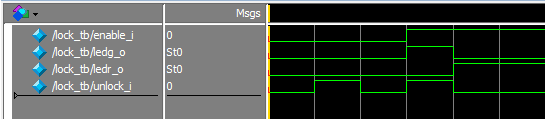
\includegraphics[width=\textwidth]{lock_sim.png}
   \caption{Testbench simulation of the lock module.}
   \label{fig:lock_sim}
\end{figure}
